\documentclass[11pt,a4paper]{report}
\usepackage[textwidth=37em,vmargin=30mm]{geometry}
\usepackage{calc,xunicode,amsmath,amssymb,paralist,enumitem,tabu,booktabs,datetime2,xeCJK,xeCJKfntef,listings}
\usepackage{tocloft,fancyhdr,tcolorbox,xcolor,graphicx,eso-pic,xltxtra,xelatexemoji}

\newcommand{\envyear}[0]{2024}
\newcommand{\envdatestr}[0]{2024-10-23}
\newcommand{\envfinaldir}[0]{webdb/2024/20241023/final}

\usepackage[hidelinks]{hyperref}
\hypersetup{
    colorlinks=false,
    pdfpagemode=FullScreen,
    pdftitle={Web Digest - \envdatestr}
}

\setlength{\cftbeforechapskip}{10pt}
\renewcommand{\cftchapfont}{\rmfamily\bfseries\large\raggedright}
\setlength{\cftbeforesecskip}{2pt}
\renewcommand{\cftsecfont}{\sffamily\small\raggedright}

\setdefaultleftmargin{2em}{2em}{1em}{1em}{1em}{1em}

\usepackage{xeCJK,xeCJKfntef}
\xeCJKsetup{PunctStyle=plain,RubberPunctSkip=false,CJKglue=\strut\hskip 0pt plus 0.1em minus 0.05em,CJKecglue=\strut\hskip 0.22em plus 0.2em}
\XeTeXlinebreaklocale "zh"
\XeTeXlinebreakskip = 0pt


\setmainfont{Brygada 1918}
\setromanfont{Brygada 1918}
\setsansfont{IBM Plex Sans}
\setmonofont{JetBrains Mono NL}
\setCJKmainfont{Noto Serif CJK SC}
\setCJKromanfont{Noto Serif CJK SC}
\setCJKsansfont{Noto Sans CJK SC}
\setCJKmonofont{Noto Sans CJK SC}

\setlength{\parindent}{0pt}
\setlength{\parskip}{8pt}
\linespread{1.15}

\lstset{
	basicstyle=\ttfamily\footnotesize,
	numbersep=5pt,
	backgroundcolor=\color{black!5},
	showspaces=false,
	showstringspaces=false,
	showtabs=false,
	tabsize=2,
	captionpos=b,
	breaklines=true,
	breakatwhitespace=true,
	breakautoindent=true,
	linewidth=\textwidth
}






\newcommand{\coverpic}[2]{
    % argv: itemurl, authorname
    Cover photo by #2~~(\href{#1}{#1})
}
\newcommand{\makeheader}[0]{
    \begin{titlepage}
        % \newgeometry{hmargin=15mm,tmargin=21mm,bmargin=12mm}
        \begin{center}
            
            \rmfamily\scshape
            \fontspec{BaskervilleF}
            \fontspec{Old Standard}
            \fontsize{59pt}{70pt}\selectfont
            WEB\hfill DIGEST
            
            \vfill
            % \vskip 30pt
            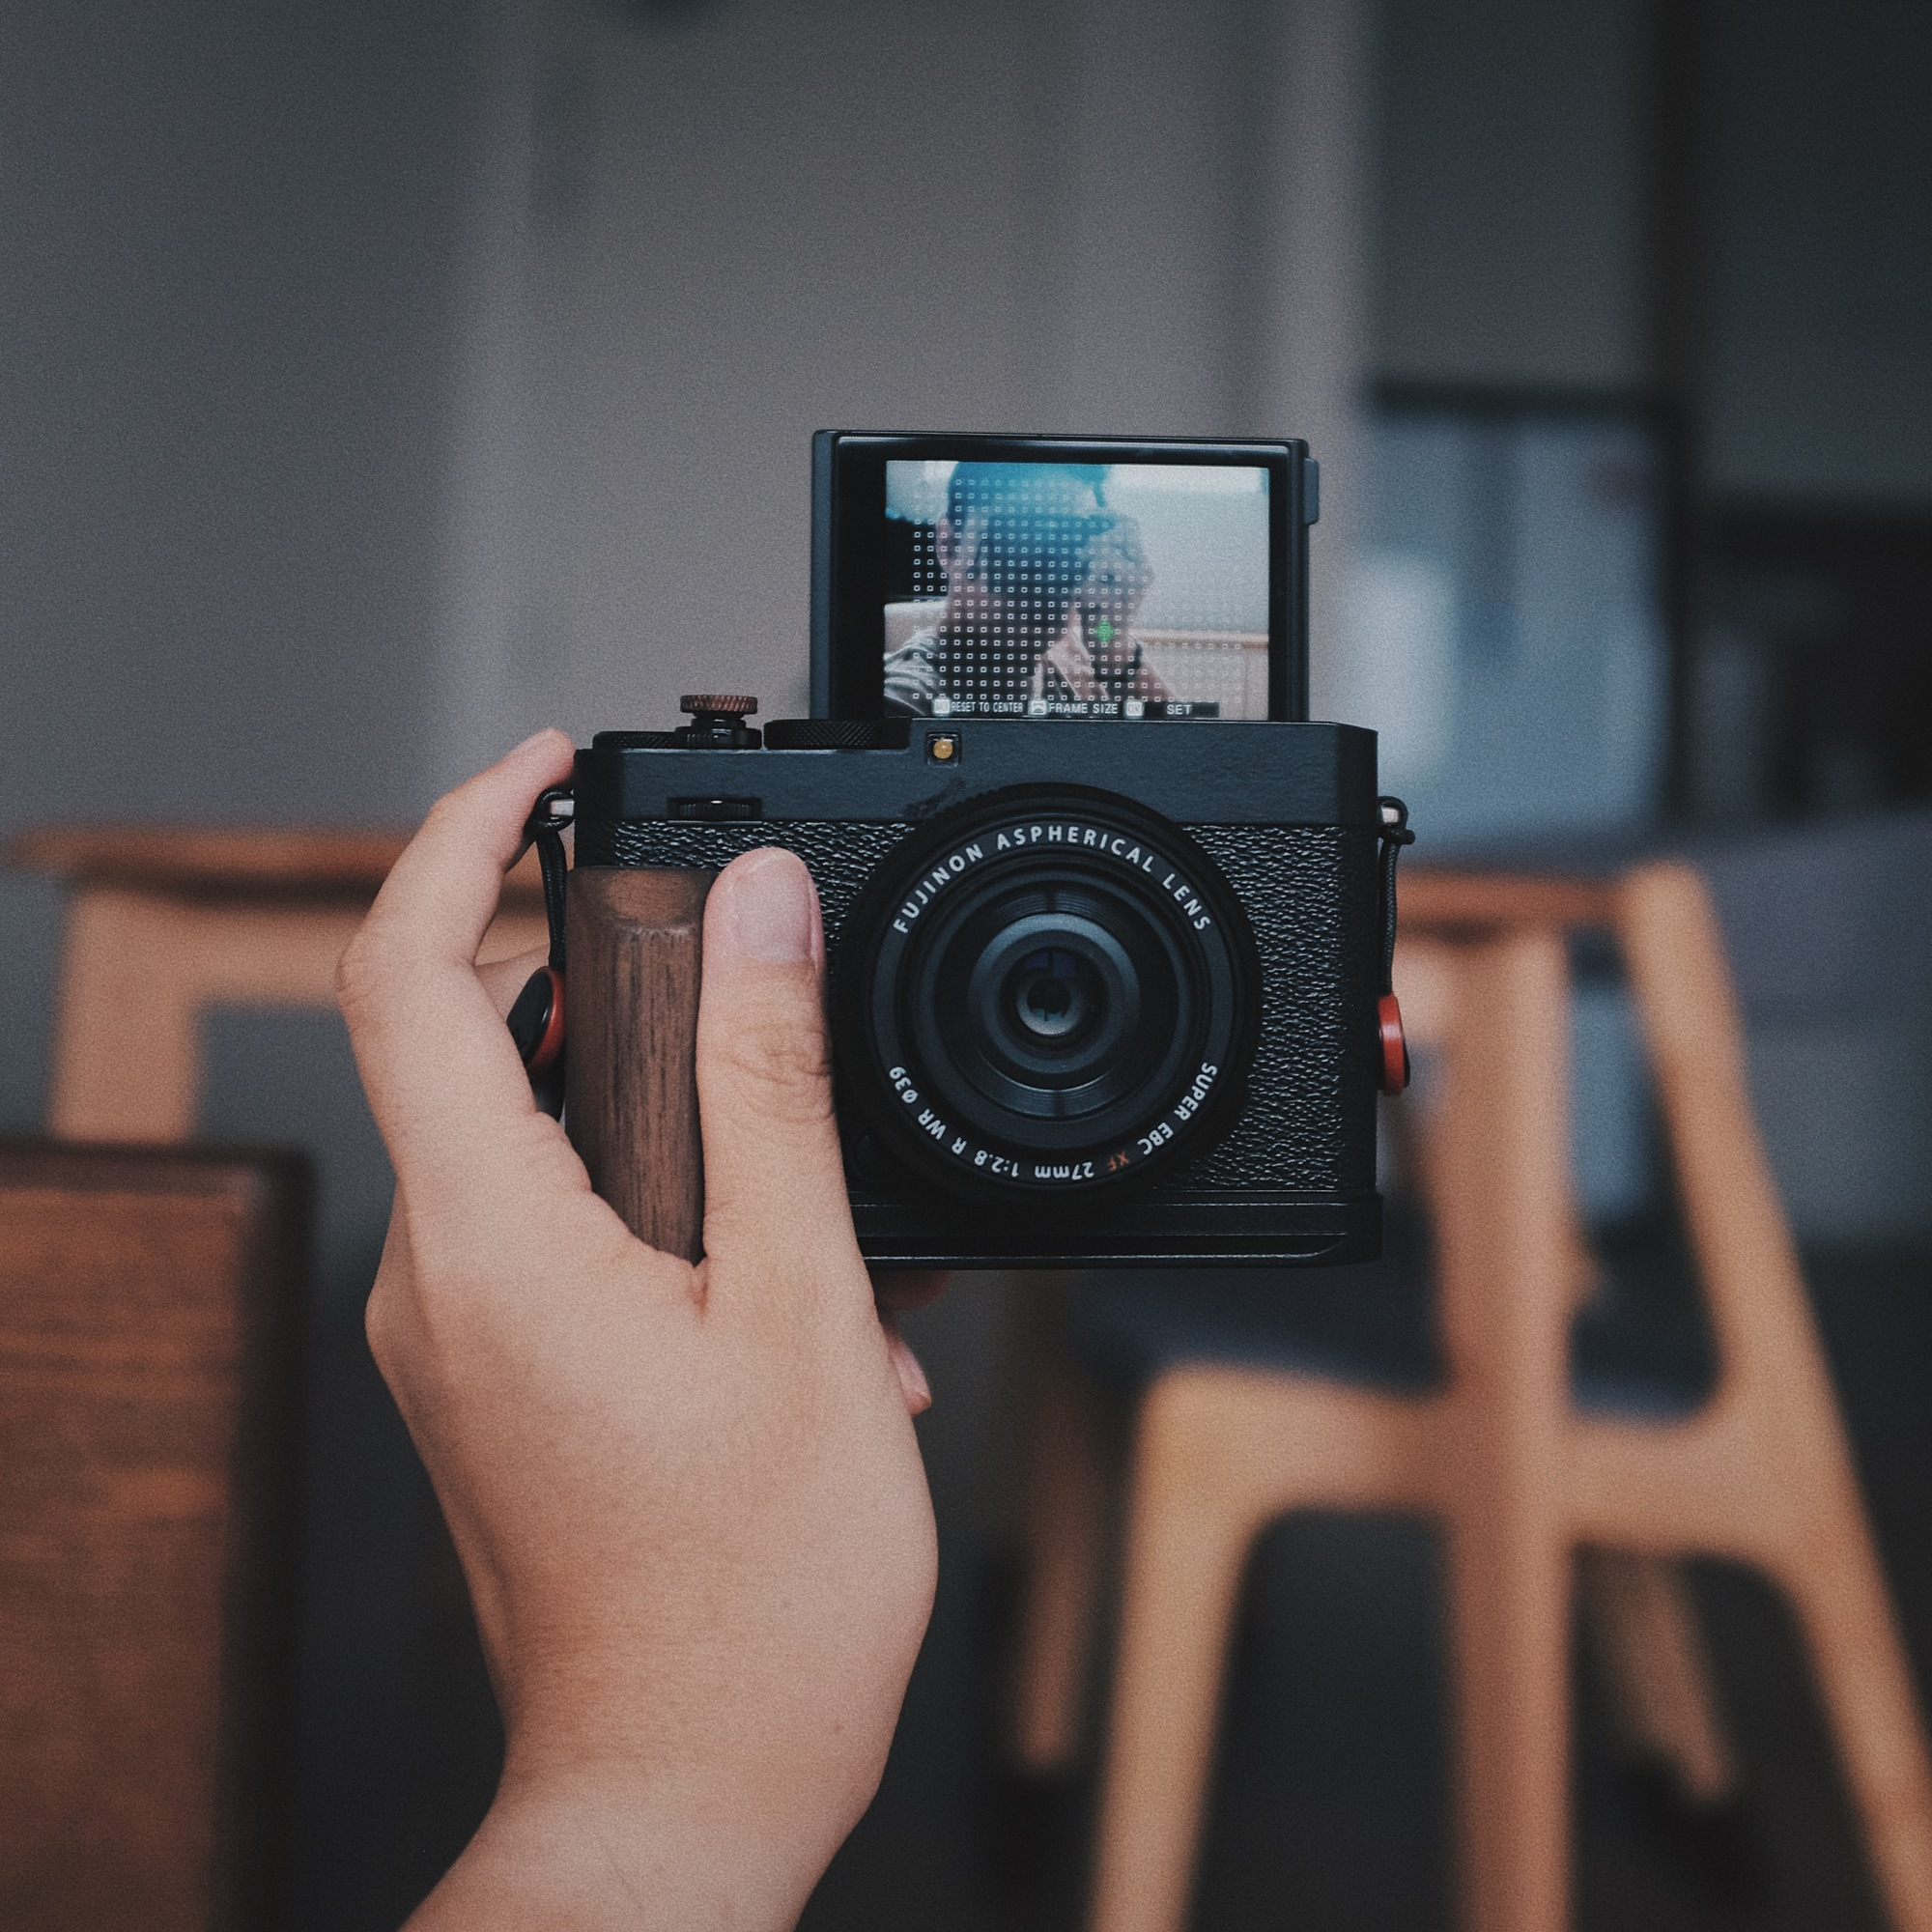
\includegraphics[width=\linewidth]{\envfinaldir/coverpic-prod.jpg}\par
            % \vskip 30pt
            \vfill

            \normalsize\rmfamily\scshape
            \copyright{} The Web Digest Project \hfill\large \envdatestr
        \end{center}
    \end{titlepage}
    % \restoregeometry
}
\newcommand{\simplehref}[1]{%
    \textcolor{blue!80!green}{\href{#1}{#1}}%
}
\renewcommand{\contentsname}{\center\Huge\sffamily\bfseries Contents\par\vskip 20pt}
\newcounter{ipartcounter}
\setcounter{ipartcounter}{0}
\newcommand{\ipart}[1]{
    % \vskip 20pt
    \clearpage
    \stepcounter{ipartcounter}
    \phantomsection
    \addcontentsline{toc}{chapter}{#1}
    % \begin{center}
    %     \Huge
    %     \sffamily\bfseries
    %     #1
    % \end{center}
    % \vskip 20pt plus 7pt
}
\newcounter{ichaptercounter}
\setcounter{ichaptercounter}{0}
\newcommand{\ichapter}[1]{
    % \vskip 20pt
    \clearpage
    \stepcounter{ichaptercounter}
    \phantomsection
    \addcontentsline{toc}{section}{\numberline{\arabic{ichaptercounter}}#1}
    \begin{center}
        \Huge
        \sffamily\bfseries
        #1
    \end{center}
    \vskip 20pt plus 7pt
}
\newcommand{\entrytitlefont}[1]{\subsection*{\raggedright\Large\sffamily\bfseries#1}}
\newcommand{\entryitemGeneric}[2]{
    % argv: title, url
    \parbox{\linewidth}{
        \entrytitlefont{#1}\par\vskip 5pt
        \footnotesize\ttfamily\mdseries
        \simplehref{#2}
    }\vskip 11pt plus 11pt minus 1pt
}
\newcommand{\entryitemGithub}[3]{
    % argv: title, url, desc
    \parbox{\linewidth}{
        \entrytitlefont{#1}\par\vskip 5pt
        \footnotesize\ttfamily\mdseries
        \simplehref{#2}\par\vskip 5pt
        \small\rmfamily\mdseries#3
    }\vskip 11pt plus 11pt minus 1pt
}
\newcommand{\entryitemAp}[3]{
    % argv: title, url, desc
    \parbox{\linewidth}{
        \entrytitlefont{#1}\par\vskip 5pt
        \footnotesize\ttfamily\mdseries
        \simplehref{#2}\par\vskip 5pt
        \small\rmfamily\mdseries#3
    }\vskip 11pt plus 11pt minus 1pt
}
\newcommand{\entryitemHackernews}[3]{
    % argv: title, hnurl, rawurl
    % \parbox{\linewidth}{
    %     \entrytitlefont{#1}\par\vskip 5pt
    %     \footnotesize\ttfamily\mdseries
    %     \simplehref{#3}\par
    %     \textcolor{black!50}{\href{#2}{#2}}
    % }\vskip 11pt plus 11pt minus 1pt
    \begin{minipage}{\linewidth}
            \entrytitlefont{#1}\par\vskip 5pt
            \footnotesize\ttfamily\mdseries
            \simplehref{#3}\par
            \textcolor{black!50}{\href{#2}{#2}}
    \end{minipage}\par\vskip 11pt plus 11pt minus 1pt
}







\begin{document}

\makeheader

\tableofcontents\clearpage




\ipart{Developers}
\ichapter{Hacker News}
\entryitemTwoLinks{Meta Bans Accounts Tracking Private Jets for Zuckerberg, Musk}{https://news.ycombinator.com/item?id=41919173}{https://www.bloomberg.com/news/articles/2024-10-22/meta-bans-accounts-tracking-private-jets-for-zuckerberg-musk}

\entryitemTwoLinks{Elderly dementia patients are unwittingly fueling political campaigns}{https://news.ycombinator.com/item?id=41918383}{https://www.cnn.com/interactive/2024/10/politics/political-fundraising-elderly-election-invs-dg/}

\entryitemTwoLinks{The Tragedy of Google Books (2017)}{https://news.ycombinator.com/item?id=41917016}{https://www.theatlantic.com/technology/archive/2017/04/the-tragedy-of-google-books/523320/}

\entryitemTwoLinks{USGS uses machine learning to show large lithium potential in Arkansas}{https://news.ycombinator.com/item?id=41916322}{https://www.usgs.gov/news/national-news-release/unlocking-arkansas-hidden-treasure-usgs-uses-machine-learning-show-large}

\entryitemTwoLinks{Show HN: Open-source Counter-Strike-like game}{https://news.ycombinator.com/item?id=41915958}{https://github.com/solcloud/Counter-Strike}

\entryitemTwoLinks{FTC's rule banning fake online reviews goes into effect}{https://news.ycombinator.com/item?id=41915187}{https://abcnews.go.com/US/wireStory/ftcs-rule-banning-fake-online-reviews-effect-115009298}

\entryitemTwoLinks{Computer use, a new Claude 3.5 Sonnet, and Claude 3.5 Haiku}{https://news.ycombinator.com/item?id=41914989}{https://www.anthropic.com/news/3-5-models-and-computer-use}

\entryitemTwoLinks{We built a new powerful JSON data type for ClickHouse}{https://news.ycombinator.com/item?id=41914845}{https://clickhouse.com/blog/a-new-powerful-json-data-type-for-clickhouse}

\entryitemTwoLinks{Show HN: Rust Web Framework}{https://news.ycombinator.com/item?id=41914544}{https://github.com/levkk/rwf}

\entryitemTwoLinks{Against /tmp}{https://news.ycombinator.com/item?id=41913610}{https://dotat.at/@/2024-10-22-tmp.html}

\entryitemTwoLinks{Tog's Paradox}{https://news.ycombinator.com/item?id=41913437}{https://www.votito.com/methods/togs-paradox/}

\entryitemTwoLinks{MQTT turns 25}{https://news.ycombinator.com/item?id=41912787}{https://andypiper.co.uk/2024/10/22/mqtt-turns-25-heres-how-it-has-endured/}

\entryitemTwoLinks{Don't Publish with IEEE (2005)}{https://news.ycombinator.com/item?id=41912625}{http://cr.yp.to/writing/ieee.html}

\entryitemTwoLinks{Understanding Gaussians}{https://news.ycombinator.com/item?id=41912160}{https://gestalt.ink/gaussians}

\entryitemTwoLinks{Singapore OKs 4,300km subsea cable for importing electricity from Australia}{https://news.ycombinator.com/item?id=41912103}{https://mothership.sg/2024/10/ema-conditional-approval-sun-cable/}

\entryitemTwoLinks{Guide to Fine-Tuning LLMs}{https://news.ycombinator.com/item?id=41911255}{https://arxiv.org/abs/2408.13296}

\entryitemTwoLinks{Firefox-Passwords-Decryptor: Extracts and decrypts passwords saved in Firefox}{https://news.ycombinator.com/item?id=41911176}{https://github.com/Sohimaster/Firefox-Passwords-Decryptor}

\entryitemTwoLinks{LTESniffer: An Open-Source LTE Downlink/Uplink Eavesdropper}{https://news.ycombinator.com/item?id=41910084}{https://github.com/SysSec-KAIST/LTESniffer}

\entryitemTwoLinks{Apple's AirPods Pro hearing health features}{https://news.ycombinator.com/item?id=41909967}{https://www.theverge.com/24275178/apple-airpods-pro-hearing-aid-test-protection-preview}

\entryitemTwoLinks{Wired's Attack on Privacy}{https://news.ycombinator.com/item?id=41909941}{https://simplex.chat/blog/20241016-wired-attack-on-privacy.html}\ichapter{Phoronix}
\entryitemGeneric{\hskip 0pt{}Rust-Written Rustls Now Reportedly Outperforming OpenSSL \& BoringSSL}{https://www.phoronix.com/news/Rustls-Faster-Than-OpenSSL}

\entryitemGeneric{\hskip 0pt{}Several Linux Kernel Driver Maintainers Removed Due To Their Association To Russia}{https://www.phoronix.com/news/Russian-Linux-Maintainers-Drop}

\entryitemGeneric{\hskip 0pt{}AlmaLinux OS Kitten 10 Now Available For Testing, Derived From CentOS Stream 10}{https://www.phoronix.com/news/AlmaLinux-Kitten-10}

\entryitemGeneric{\hskip 0pt{}System76 Thelio Astra Reviewed: High-End ARM64 Developer Desktop}{https://www.phoronix.com/review/system76-thelio-astra}

\entryitemGeneric{\hskip 0pt{}NVIDIA R565 Linux Driver Beta Brings Improvements For Wayland, DMA-BUF \& VKD3D}{https://www.phoronix.com/news/NVIDIA-565.57.01-Linux-Beta}

\entryitemGeneric{\hskip 0pt{}Intel Preps GCC Compiler For New AMX \& ISA Features Ahead Of Diamond Rapids}{https://www.phoronix.com/news/Intel-GCC-Diamond-Rapids-ISA}

\entryitemGeneric{\hskip 0pt{}Intel Compute Runtime 24.39.31294.12 Fixes Lunar Lake OpenCL, Disables Ice Lake \& Older}{https://www.phoronix.com/news/Intel-CR-24.39.31294.12}

\entryitemGeneric{\hskip 0pt{}Suggestion Raised For Using PGO + LLVM BOLT To Optimize More Fedora Packages}{https://www.phoronix.com/news/Fedora-Idea-More-PGO-LLVM-BOLT}

\entryitemGeneric{\hskip 0pt{}Wasmer 5.0-rc1 Adds Experimental Support For WASMI, Interpreter Mode Support}{https://www.phoronix.com/news/Wasmer-5.0-rc1}


\ipart{Developers~~~~(zh-Hans)}
\ichapter{Solidot}
\entryitemGeneric{\hskip 0pt{}Google Scholar 认证了牛顿爵士的电邮}{https://www.solidot.org/story?sid=79559}

\entryitemGeneric{\hskip 0pt{}李彦宏预测 AI 是另一个泡沫,99\% 的 AI 公司会在泡沫破裂时面临倒闭}{https://www.solidot.org/story?sid=79558}

\entryitemGeneric{\hskip 0pt{}《Squadron 42》将于 2026 年发布}{https://www.solidot.org/story?sid=79557}

\entryitemGeneric{\hskip 0pt{}被裁的 IT 员工变成前雇主的 IT 外包}{https://www.solidot.org/story?sid=79556}

\entryitemGeneric{\hskip 0pt{}前英伟达工程师发现第 52 个梅森素数}{https://www.solidot.org/story?sid=79555}

\entryitemGeneric{\hskip 0pt{}微软屏蔽两款华硕笔记本更新 Windows 11 24H2}{https://www.solidot.org/story?sid=79554}

\entryitemGeneric{\hskip 0pt{}AI 关键词更可能增加论文引用率}{https://www.solidot.org/story?sid=79553}

\entryitemGeneric{\hskip 0pt{}埃及消灭了疟疾}{https://www.solidot.org/story?sid=79552}

\entryitemGeneric{\hskip 0pt{}政治自恋助长了将政治对手非人化的倾向}{https://www.solidot.org/story?sid=79551}

\entryitemGeneric{\hskip 0pt{}大黄蜂蜂后选择在农药污染的土壤下冬眠}{https://www.solidot.org/story?sid=79550}

\entryitemGeneric{\hskip 0pt{}X 的竞争对手 Bluesky 两天增加 120 万新用户}{https://www.solidot.org/story?sid=79549}

\entryitemGeneric{\hskip 0pt{}Linux 6.13 预计将移除 ReiserFS 文件系统}{https://www.solidot.org/story?sid=79548}

\entryitemGeneric{\hskip 0pt{}GNU Boot 再次发现包含非自由代码}{https://www.solidot.org/story?sid=79547}

\entryitemGeneric{\hskip 0pt{}字节跳动以恶意干扰 AI 模型训练为由解雇了一名实习生}{https://www.solidot.org/story?sid=79546}

\entryitemGeneric{\hskip 0pt{}更多证据表明长新冠是一种脑损伤}{https://www.solidot.org/story?sid=79545}

\entryitemGeneric{\hskip 0pt{}微软用蜜罐大规模欺骗钓鱼者}{https://www.solidot.org/story?sid=79544}

\entryitemGeneric{\hskip 0pt{}在致命车祸后美国调查特斯拉的 Full Self-Driving 软件}{https://www.solidot.org/story?sid=79543}

\entryitemGeneric{\hskip 0pt{}Ubuntu 发布二十周年}{https://www.solidot.org/story?sid=79542}

\entryitemGeneric{\hskip 0pt{}芯片设计师回顾了英特尔和 AMD 之间围绕 x86-64 的竞争}{https://www.solidot.org/story?sid=79541}

\entryitemGeneric{\hskip 0pt{}古巴大范围断电已持续三天}{https://www.solidot.org/story?sid=79540}\ichapter{V2EX}
\entryitemGeneric{\hskip 0pt{}[问与答] HarmonyOS NEXT 连内核都是自研的?}{https://www.v2ex.com/t/1082730}

\entryitemGeneric{\hskip 0pt{}[宽带症候群] 想要在 macOS 上做 CCIE 的路由和交换实验,请问目前什么模拟器最合适?(没有真机环境)}{https://www.v2ex.com/t/1082729}

\entryitemGeneric{\hskip 0pt{}[程序员] 九号 MZmix 第一次远足}{https://www.v2ex.com/t/1082728}

\entryitemGeneric{\hskip 0pt{}[酷工作] [Remote] Prompt Engineering / AI 工程师 / Prompt 工程师}{https://www.v2ex.com/t/1082727}

\entryitemGeneric{\hskip 0pt{}[Apple] 请教大家,如果出二手设备会被导致 id 被连坐封号吗?}{https://www.v2ex.com/t/1082725}

\entryitemGeneric{\hskip 0pt{}[程序员] 公司财务服务器用的三星 850 PRO 通电已经 81656 小时了,写入才 27.8TBW,有必要换掉吗?没有组 RAID,备份只有按天的}{https://www.v2ex.com/t/1082724}

\entryitemGeneric{\hskip 0pt{}[问与答] 2024 年大家最常用的 Windows 和 Android 代理软件有哪些}{https://www.v2ex.com/t/1082722}

\entryitemGeneric{\hskip 0pt{}[OpenAI] Claude 3.5 Haiku 模型发布! Claude 3.5 Sonnet 重大升级,可操作计算机}{https://www.v2ex.com/t/1082721}

\entryitemGeneric{\hskip 0pt{}[Android] 下部手机买什么啊?}{https://www.v2ex.com/t/1082720}

\entryitemGeneric{\hskip 0pt{}[问与答] 求推荐好用的收藏夹同步工具}{https://www.v2ex.com/t/1082719}

\entryitemGeneric{\hskip 0pt{}[职场话题] offer 选择迷茫}{https://www.v2ex.com/t/1082718}

\entryitemGeneric{\hskip 0pt{}[酷工作] 远程工作 Java 前端各一个}{https://www.v2ex.com/t/1082717}

\entryitemGeneric{\hskip 0pt{}[程序员] 问一下各位佬 b 站 up 主首页的搜索视频模块是怎么做的?为什么匹配的字段会搜不到?}{https://www.v2ex.com/t/1082716}

\entryitemGeneric{\hskip 0pt{}[问与答] 查询 iOS App 历史版本对应的 ID 有哪些渠道?}{https://www.v2ex.com/t/1082715}

\entryitemGeneric{\hskip 0pt{}[宽带症候群] Mac 上用的科学软件,除了 Clash, 还有别的推荐吗?}{https://www.v2ex.com/t/1082713}

\entryitemGeneric{\hskip 0pt{}[分享创造] V 站有从事线上运营推广的铁子吗,可以找我领福利}{https://www.v2ex.com/t/1082712}

\entryitemGeneric{\hskip 0pt{}[程序员] 求助 Windows 局域网共享仅能设置所有人都可访问,无法设置密码保护}{https://www.v2ex.com/t/1082711}

\entryitemGeneric{\hskip 0pt{}[MacBook Pro] 个人预测 Macbook 新品发布时间}{https://www.v2ex.com/t/1082710}

\entryitemGeneric{\hskip 0pt{}[程序员] 急需一个久坐监控}{https://www.v2ex.com/t/1082707}

\entryitemGeneric{\hskip 0pt{}[职场话题] 大厂 vs 研究所, offer 选择求助}{https://www.v2ex.com/t/1082706}

\entryitemGeneric{\hskip 0pt{}[Flutter] 造个小轮子,开源一个 Flutter 的业务需求常见功能组件, TabBar 锚点自动定位 ScrollView}{https://www.v2ex.com/t/1082705}

\entryitemGeneric{\hskip 0pt{}[分享创造] 我对信息流应用的思考 [build in public]}{https://www.v2ex.com/t/1082704}

\entryitemGeneric{\hskip 0pt{}[酷工作] [全职/实习招聘-坐班上海] Narya.ai | AI 应用赛道 | 急招 iOS 开发 | 月薪 40~ 60K+ RMB}{https://www.v2ex.com/t/1082703}

\entryitemGeneric{\hskip 0pt{}[iCloud] iCloud 国区合租 季付 36}{https://www.v2ex.com/t/1082702}

\entryitemGeneric{\hskip 0pt{}[酷工作] 美国初创公司线上办公招聘工程师}{https://www.v2ex.com/t/1082700}

\entryitemGeneric{\hskip 0pt{}[问与答] 二开了一个数据库管理工具怎么基于 vscode-oss 打包成独立客户端}{https://www.v2ex.com/t/1082699}

\entryitemGeneric{\hskip 0pt{}[程序员] 一起读书: Computer Organization and Design RISC-V Edition}{https://www.v2ex.com/t/1082698}

\entryitemGeneric{\hskip 0pt{}[iCloud] icloud2t 家庭车拼车 Q1,一月 10/ 400g}{https://www.v2ex.com/t/1082697}

\entryitemGeneric{\hskip 0pt{}[职场话题] 正规菠菜公司的 offer 要不要接,但是发 USTD}{https://www.v2ex.com/t/1082696}

\entryitemGeneric{\hskip 0pt{}[Android] 手机电池疑似故障,这种情况还有救吗}{https://www.v2ex.com/t/1082695}

\entryitemGeneric{\hskip 0pt{}[云计算] 腾讯云账号 企业账号 实名账号 可关联 可首单 防丢防找回}{https://www.v2ex.com/t/1082694}

\entryitemGeneric{\hskip 0pt{}[汽车] 说个我自己买车的趣事}{https://www.v2ex.com/t/1082693}

\entryitemGeneric{\hskip 0pt{}[职场话题] 有 web 前端转 Go 或 C++经验的前辈吗}{https://www.v2ex.com/t/1082691}

\entryitemGeneric{\hskip 0pt{}[Android] 求推荐几款可以 root,可以 google pay 的手机}{https://www.v2ex.com/t/1082690}

\entryitemGeneric{\hskip 0pt{}[酷工作] kimi 搜索团队招工程,算法}{https://www.v2ex.com/t/1082689}

\entryitemGeneric{\hskip 0pt{}[Apple] mac 上来自 iPhone 的通知怎么这么少,连微信通知都没有了}{https://www.v2ex.com/t/1082688}

\entryitemGeneric{\hskip 0pt{}[职场话题] 大家觉得搞物联网有前途,还是互联网}{https://www.v2ex.com/t/1082686}

\entryitemGeneric{\hskip 0pt{}[问与答] 请问上海有无合约机套餐推荐?}{https://www.v2ex.com/t/1082684}

\entryitemGeneric{\hskip 0pt{}[问与答] V 友们,有没有辅助写可研、项目建议书这类报告的工具。}{https://www.v2ex.com/t/1082681}

\entryitemGeneric{\hskip 0pt{}[宽带症候群] 每晚八点开始,跨运营商限速}{https://www.v2ex.com/t/1082680}

\entryitemGeneric{\hskip 0pt{}[宽带症候群] 现在还存在 T1/E1 吗}{https://www.v2ex.com/t/1082679}

\entryitemGeneric{\hskip 0pt{}[问与答] 想问一下这两个需求是不是冷门需求(连环画、国内风景)}{https://www.v2ex.com/t/1082677}

\entryitemGeneric{\hskip 0pt{}[Apple] 安卓党换 iphone16pm 后的一些不适}{https://www.v2ex.com/t/1082676}

\entryitemGeneric{\hskip 0pt{}[VXNA] 申请收录博客: heggria}{https://www.v2ex.com/t/1082674}

\entryitemGeneric{\hskip 0pt{}[问与答] 别人都觉得我很顺利,羡慕之类的话。}{https://www.v2ex.com/t/1082673}

\entryitemGeneric{\hskip 0pt{}[分享发现] 推荐一个机场}{https://www.v2ex.com/t/1082672}

\entryitemGeneric{\hskip 0pt{}[Apple] 换了一阵子 AirPods 4 降噪版,分享下主观感受}{https://www.v2ex.com/t/1082671}

\entryitemGeneric{\hskip 0pt{}[问与答] 如何优雅地切换 ios app store 国区 美区 账号?}{https://www.v2ex.com/t/1082670}

\entryitemGeneric{\hskip 0pt{}[生活] 求分享一个好习惯和一个好消遣}{https://www.v2ex.com/t/1082669}

\entryitemGeneric{\hskip 0pt{}[酷工作] 个人项目招聘 ios 客户端一名}{https://www.v2ex.com/t/1082668}


\ipart{Generic News}
\ichapter{AP News}
\entryitemWithDescription{\hskip 0pt{}Trump will conduct an interview with Joe Rogan for his podcast}{https://apnews.com/article/b89e4c021df206208dc19f78dc811828}{}

\entryitemWithDescription{\hskip 0pt{}ABBA, Radiohead and The Cure musicians sign AI protest letter against `unlicensed use' of works}{https://apnews.com/article/ba9091a6095876affe8c09f6bf9fe12d}{}

\entryitemWithDescription{\hskip 0pt{}A\$AP Rocky to go to trial next year on charges he fired a gun at a former friend}{https://apnews.com/article/8137161cb7438e41b3fe6e33f8e41ba2}{}

\entryitemWithDescription{\hskip 0pt{}Denny's says it expects to close 150 locations by the end of 2025}{https://apnews.com/article/68a38e40337f4650425c45069997b875}{}

\entryitemWithDescription{\hskip 0pt{}Flying air taxis move closer to US takeoff with issuing of FAA rule}{https://apnews.com/article/85fd3c8b905a003eff64590afb5da339}{}

\entryitemWithDescription{\hskip 0pt{}A New Zealand airport wants you to hug goodbye faster}{https://apnews.com/article/d6176082ffb6ab66e8d2f05dd590b8aa}{}

\entryitemWithDescription{\hskip 0pt{}`Blade Runner 2049' producers sue Elon Musk and Tesla over AI image at robotaxi event}{https://apnews.com/article/384c0fbdc536d0c5cfc13794507c3b9f}{}

\entryitemWithDescription{\hskip 0pt{}No rugby, field hockey, badminton, triathlon or cricket at leaner 2026 Commonwealth Games}{https://apnews.com/article/ad279947a74b1371fb372285e160e738}{}

\entryitemWithDescription{\hskip 0pt{}King Charles III's Commonwealth visit to Samoa will highlight climate change ... and dance}{https://apnews.com/article/89b658cf3b0529b7a19c0361208a29c8}{}

\entryitemWithDescription{\hskip 0pt{}Georgia Supreme Court reverses contempt ruling against rapper Young Thug's lawyer}{https://apnews.com/article/86b16d60003cb640e4f7e3f7587958e9}{}

\entryitemWithDescription{\hskip 0pt{}Initial report shows Liam Payne had cocaine in his system when he died, says Argentine official}{https://apnews.com/article/dae90a8090a46cf4af72d8fe359f38df}{}

\entryitemWithDescription{\hskip 0pt{}Facing 7 more lawsuits, Sean `Diddy' Combs protests a `fresh wave of publicity'}{https://apnews.com/article/0c25d256ee9351a64c30a8398c5a46d4}{}

\entryitemWithDescription{\hskip 0pt{}Duke's Cooper Flagg makes preseason AP All-America team as ACC, Big 12, SEC each place 2 players}{https://apnews.com/article/2b6f3922ae1bee8c6f8c8bb71449e2b1}{}\ichapter{Reuters}
\entryitemWithDescription{\hskip 0pt{}Capitol riot defendants face upheld trespassing charges in US court}{https://www.reuters.com/legal/capitol-riot-defendants-face-upheld-trespassing-charges-us-court-2024-10-22/}{A U.S. appeals court on Tuesday upheld the use of a criminal trespassing charge against nearly all of the 1,500 defendants accused of taking part in the Jan. 6, 2021, attack on the U.S. Capitol, rejecting an attempt to further restrict...}

\entryitemWithDescription{\hskip 0pt{}Israel's military confirms killing of Lebanon Hezbollah's Hashem Safieddine}{https://www.reuters.com/world/middle-east/israels-military-confirms-killing-lebanon-hezbollahs-hashem-safieddine-2024-10-22/}{Israel\textquotesingle s military confirmed on Tuesday the killing of Hashem Safieddine, of Lebanon\textquotesingle s Hezbollah, who is the apparent heir to Hassan Nasrallah, who was killed in an Israeli...}

\entryitemWithDescription{\hskip 0pt{}Blinken told Netanyahu Israel needs to do more on Gaza humanitarian aid}{https://www.reuters.com/world/blinken-told-netanyahu-israel-needs-do-more-gaza-humanitarian-aid-2024-10-22/}{U.S. Secretary of State Antony Blinken told Israeli Prime Minister Benjamin Netanyahu on Tuesday that Israel has so far taken insufficient steps to get more humanitarian aid into Gaza, and he asked it to work to improve the situation, a...}

\entryitemWithDescription{\hskip 0pt{}Peru to scrutinize Venezuelan remittances amid crime concerns}{https://www.reuters.com/world/americas/peru-monitor-venezuelan-migrants-remittances-amid-crime-fears-2024-10-22/}{Peru\textquotesingle s government will monitor money transfers sent abroad from Venezuelans living in Peru, President Dina Boluarte announced on Tuesday, describing the measure as a response to rising crime that she linked to Venezuelan...}

\entryitemWithDescription{\hskip 0pt{}In Havana's still dark corners, a protest erupts}{https://www.reuters.com/world/americas/havanas-still-dark-corners-protest-erupts-2024-10-22/}{Just three or four city blocks in all of Central Havana remained without electricity on Monday evening - an island of darkness in the Cuban capital\textquotesingle s sea of flashing lights, pounding reggaeton and jammed bars and...}

\entryitemWithDescription{\hskip 0pt{}Drone attack in northern Mali kills at least 8, Tuareg rebels say}{https://www.reuters.com/world/africa/drone-attack-northern-mali-kills-least-8-tuareg-rebels-say-2024-10-22/}{At least eight people including children were killed and 20 injured in a drone strike at a fair in Mali\textquotesingle s northern Timbuktu region, Tuareg rebels said on...}

\entryitemWithDescription{\hskip 0pt{}Zelenskiy calls on allies 'not to hide', respond to N.Korean involvement in war}{https://www.reuters.com/world/zelenskiy-calls-allies-not-hide-respond-nkorean-involvement-war-2024-10-22/}{Ukrainian President Volodymyr Zelenskiy called on allies on Tuesday "not to hide" and to respond to evidence of North Korean involvement into Russia\textquotesingle s war in...}

\entryitemWithDescription{\hskip 0pt{}US, G7 allies 'very close' to finalizing \$50 billion Ukraine loan, Yellen says}{https://www.reuters.com/world/us-g7-allies-very-close-finalizing-50-billion-ukraine-loan-yellen-says-2024-10-22/}{U.S. Treasury Secretary Janet Yellen said on Tuesday that G7 and European Union allies are "very close" to finalizing a \$50 billion loan to Ukraine backed by frozen Russian assets, with an expected U.S. contribution of about \$20...}

\entryitemWithDescription{\hskip 0pt{}Argentina prosecutor: Liam Payne lab reports ongoing, results needed to release body}{https://www.reuters.com/world/americas/argentina-prosecutor-liam-payne-lab-reports-ongoing-results-needed-release-body-2024-10-22/}{An Argentina prosecutor said on Tuesday that toxicological and other laboratory reports into the death of former One Direction singer Liam Payne were not yet completed, with the results needed to release the body to his...}

\entryitemWithDescription{\hskip 0pt{}Ireland seeks to limit trade with Israeli settlements in occupied territories}{https://www.reuters.com/world/ireland-seeks-way-restrict-trade-with-occupied-palestinian-territories-2024-10-22/}{Ireland\textquotesingle s government is seeking to introduce a bill restricting trade with Israeli settlements in the occupied Palestinian territories after it said a UN court decision freed Dublin to make trade decisions independently of...}

\entryitemWithDescription{\hskip 0pt{}US charges IRGC official, others in Iran-backed plot to assassinate journalist}{https://www.reuters.com/world/us-charges-irgc-official-others-iran-backed-plot-assassinate-journalist-2024-10-22/}{The United States issued fresh charges over the attempted Tehran plot to kidnap and assassinate an Iranian-American journalist in New York, indicting an Iranian Revolutionary Guards Corps (IRGC) official among others in the case...}

\entryitemWithDescription{\hskip 0pt{}Netanyahu meets Blinken, urges political and security changes in Lebanon}{https://www.reuters.com/world/middle-east/netanyahu-meets-blinken-urges-political-security-changes-lebanon-2024-10-22/}{Israeli Prime Minister Benjamin Netanyahu, meeting with U.S. Secretary of State Antony Blinken, said there was a need for a security and political change in Lebanon that would allow displaced Israelis to return safely to their...}

\entryitemWithDescription{\hskip 0pt{}Ukraine's prosecutor general resigns amid draft-dodging scandal}{https://www.reuters.com/world/europe/ukraines-prosecutor-general-andriy-kostin-resigns-amid-draft-dodging-scandal-2024-10-22/}{Ukraine\textquotesingle s Prosecutor General Andriy Kostin said on Tuesday he had resigned to take responsibility for a scandal in which dozens of officials are alleged to have abused their position to receive disability status and avoid...}\ichapter{联合早报}
\entryitemWithDescription{沈泽玮:台湾冲突阻遏法案只叫不咬?}{https://www.zaobao.com/news/china/story20240918-4758889}{美国众议院9月9日开启了长达一星期的``中国周'',共通过25项主要涉华法案。(法新社) 美国众议院在当地时间9月9日开启了长达一星期的``中国周'',在美国总统和国会选举举行之前,密集表决数十项与中国有关的法案,共通过25项主要涉华法案……}

\entryitemWithDescription{欧盟电动车关税投票倒计时 中国在分歧中寻支持}{https://www.zaobao.com/news/china/story20240917-4758953}{欧盟27个成员国将于9月25日就是否继续对进口自中国的电动汽车额外征税进行最后表决。图为上海港等待装运出口的电动汽车。(彭博社) 欧盟对中国电动汽车加征关税的投票进入倒计时,正在欧洲访问的中国商务部部长王文涛与欧盟多国政府高层就此进行协商,试图在立场分歧的成员国中争取到更多支持。 受访学者研判,欧盟对中国电动汽车加征关税不可避免,但具体的加税方式和幅度仍有一定弹性,这是王文涛此行与各国谈判的重点……}

\entryitemWithDescription{港府今年将举办逾400项国庆活动}{https://www.zaobao.com/news/china/story20240917-4759341}{再过十多天就是中国国庆75周年,香港天星小轮展示``国庆75周年''\,``三天免费搭小轮''等标语迎国庆。(中新社) 再过十多天就是中国国庆75周年,香港特区政府今年将举办逾400项庆祝活动,希望通过一连串活动庆祝国庆,并且弘扬爱国主义教育及刺激消费。 港府星期二(9月17日)召开记者会,介绍各项庆祝国庆活动和特别优惠,涉及出行及吃喝玩乐等领域……}

\entryitemWithDescription{美空军部长:中国大陆军演精密化 为入侵封锁台湾做准备}{https://www.zaobao.com/news/china/story20240917-4759407}{美国空军部长肯德尔星期一(9月16日)在空军暨太空军协会的一场大会上致辞,提到中国对印太地区日益增长的威胁。(取自美国国防部网站) (华盛顿综合讯)美国空军部长肯德尔指,中国大陆军演的规模越来越大,也更加精密化,这是在专门为入侵、封锁台湾做准备。他也称,中国对印太地区的威胁现在已存在……}

\entryitemWithDescription{批准潜在对台备件军售案后 美派巡逻机过航台海}{https://www.zaobao.com/news/china/story20240917-4758770}{台军士兵8月26日在屏东县枋山训练场进行实弹演习时,从M1167 TOW运载车上发射一枚美制TOW-2A线导反坦克导弹。(路透社) (华盛顿/台北/北京综合讯)在批准潜在对台备件军售案之后,美国派遣反潜巡逻机过航台湾海峡,中国人民解放军东部战区则组织战机跟监美机,并誓言``坚决捍卫国家主权''……}

\entryitemWithDescription{李家超:若香港驻美经贸办被关 受害的是美企}{https://www.zaobao.com/news/china/story20240917-4758797}{香港特首李家超星期一(9月17日)警告,如果美国通过法案,导致香港驻美经贸办关闭,受害的是美国企业。图为李家超9月11日在``一带一路''高峰论坛上致辞。(彭博社) (香港综合讯)香港特首李家超警告,如果美国通过法案,导致香港驻美经贸办关闭,受害的是美国企业。 美国众议院上周通过《香港经济贸易办事处认证法案》,如果参议院也表决通过并交由总统签署成法,香港三个驻美国的经贸办可能将被强制关闭……}

\entryitemWithDescription{美国指中国航空工业集团员工企图实施黑客攻击}{https://www.zaobao.com/news/china/story20240917-4757988}{(华盛顿综合讯)中国航空航天巨头中国航空工业集团一名员工被指试图对美国宇航局、美国军方和其他目标展开黑客攻击。 据彭博社报道,美国检察官布坎南星期一(9月16日)在起诉书中,指控中国航空工业集团39岁的工程师吴宋(音译,Song Wu)企图从美国宇航局、空军、陆军和海军,以及联邦航空管理局取得电脑软件和源代码……}

\entryitemWithDescription{【东谈西论】恒大账务造假 普华永道是共犯还是被拖累?}{https://www.zaobao.com/news/china/story20240917-4756452}{因涉及恒大地产审计项目的违法行为,普华永道中国9月13日被中国财政部和证监会处以4.41亿人民币罚款并被令停业六个月, 广州分所被撤销……}

\entryitemWithDescription{戴庆成:香港输入人才计划大检阅}{https://www.zaobao.com/news/china/story20240917-4744978}{香港于2022年底推出高端人才通行证计划。(法新社) 2019年香港反修例风波过后,数以十万计港人移居海外,令香港出现人才荒。港府为了解决这个问题,在过去几年积极引入``新血'',当中以高才通计划最受瞩目,社会上也不时热议其成效。 高才通全称为高端人才通行证计划,于2022年底推出,申请人年收入须达到250万港元(约42万新元)以上,或本科毕业于全球百强大学并满足一定工作年限等……}

\entryitemWithDescription{中美希望稳定双边关系 中小国家可​​​搭建桥梁}{https://www.zaobao.com/news/china/story20240917-4745091}{中美元首去年11月在旧金山会晤后,双方都希望稳定两国关系,我国巡回大使陈庆珠认为,如果中美两国都认为走向战争不符合它们的利益,那么中小国家就可以做点什么,为双方搭建桥梁。 陈庆珠星期一(9月16日)在李光耀公共政策学院的一场研讨会上说,中国与西方的关系面对诸多困难,有中国智库表示,希望新加坡能协助在中美之间建立更多对话,``因为新加坡受美国信任,也在中国有渠道''……}

\entryitemWithDescription{陈庆珠:世界经历了三次``中国冲击'' 中美的主导力之争将继续}{https://www.zaobao.com/news/china/story20240917-4744996}{李光耀公共政策学院``思想之节庆''的一场研讨会,讨论``历史终结时的中国冲击''。左起是我国巡回大使陈庆珠、通商中国主席李奕贤、李光耀公共政策学院国际关系助理教授何莉菁、李光耀公共政策学院院长柯成兴……}

\entryitemWithDescription{上海遭遇75年来最强台风 扰乱民众中秋假期出行}{https://www.zaobao.com/news/china/story20240916-4745224}{台风贝碧嘉星期一(9月16日)登陆上海,维护人员星期一下午在衡山路上处理倒伏的树木。 (新华社) 台风造成上海上万株数目倒伏或折断。图为一棵倒下的大树砸坏一旁的建筑。(法新社) 台风贝碧嘉登陆上海后,黄浦江苏州河口潮位上涨,乌云密布。(中新社) 中国上海市星期一(9月16日)遭遇75年来最强台风``贝碧嘉''登陆,也是上海有记录以来首次有强台风侵袭……}

\entryitemWithDescription{陆男频长驱偷渡台湾在测试边防实力?}{https://www.zaobao.com/news/china/story20240916-4745161}{中国大陆一名王姓男子在中秋节前夕,乘橡皮艇从浙江宁波抵达台湾新北市林口,主动打电话投案,海巡署人员前去接他上岸。(自由時報) 中国大陆一名王姓男子划橡皮艇于上星期六清晨偷渡到台湾,隔天被新北市地方法院裁定羁押禁见。这是6月以来第二起大陆人士偷渡至台湾,此间专家质疑是否为海防破口,并怀疑对岸是否在测试台湾的边防实力……}

\entryitemWithDescription{中美时隔八月举行国防部工作会晤}{https://www.zaobao.com/news/china/story20240916-4745025}{(北京/华盛顿综合讯)中美双方上周末举行国防部工作会晤;美国官员称,美国积极进行美中两军外交活动,不代表美国对有关中国议题的处理方式发生任何改变。 据中国国防部星期天(15日)晚上通报,北京香山论坛结束后,第18次中美国防部工作会晤上星期六至星期天(9月14日至15日)在北京举行……}

\entryitemWithDescription{中国高校今年拟增足球运动本科专业}{https://www.zaobao.com/news/china/story20240916-4744925}{(北京综合讯)为了培养足球专业人才,中国大专学府今年度拟新增足球运动本科专业,以具体落实中国足球改革。 综合人民网和《南方都市报》报道,中国教育部上星期五(9月13日)发布《2024年度普通高等学校本科专业申报材料公示》。根据公示统计,今年度拟新增专业535个,涉及353所高校,其中39所高校新增足球运动专业……}

\entryitemWithDescription{香港23条首案 港男因穿``光时''上衣被定罪}{https://www.zaobao.com/news/china/story20240916-4743439}{(香港综合讯)香港一名无业男子,今年6月因穿印有2019年反修例抗争口号的上衣而被捕。他星期一承认违反煽动意图罪,成为在《维护国家安全条例》(即《香港基本法》第23条)下被定罪的第一人。 综合港媒《星岛日报》和路透社报道,27岁无业男子诸启邦今年6月12日在石门港铁站附近,未能出示身份证供查阅被警方拘捕……}

\entryitemWithDescription{美国务院:中国释放被关押近20年美籍牧师}{https://www.zaobao.com/news/china/story20240916-4744614}{(华盛顿综合电)中国释放被关押近20年的美国籍牧师,显示北京在中美关系的关键时刻展现善意。 综合彭博社、法新社和路透社报道,美国国务院发言人星期天(9月15日)说:``我们欢迎林大卫(音译,David Lin)从中华人民共和国的监狱获释。他已回返美国,这是他近20年来首次与家人见面。'' 林大卫的女儿艾丽斯告诉美国政治新闻网Politico,她的父亲将抵达得克萨斯州的圣安东尼奥……}

\entryitemWithDescription{中国驻泰使馆:近期并未向湄公河下游泄洪}{https://www.zaobao.com/news/china/story20240916-4743917}{(北京讯)泰国西北部的湄公河因洪水泛滥而决堤,中国否认这是中方泄洪所致,并称近来已持续减少云南景洪水电站的出库流量,以助下游地区抗洪。 中国驻泰国大使馆星期日(9月15日)深夜在官方微信公众号发文说,当天又有媒体报道称中国正在向湄公河泄洪,经向中国主管部门核实,使馆再次澄清,为帮助下游地区应对洪灾,中方近来持续稳定和减少景洪水电站出库流量,不可能对下游地区抗洪救灾形成压力……}

\entryitemWithDescription{加入美国储存可靠度评估计划 台湾军方编列预算采购三类型导弹}{https://www.zaobao.com/news/china/story20240916-4743826}{(台北讯)据台媒报道,台湾军方持续向美国采购可简易操作的导弹,预计在2024年、2031年以前获得400枚``标枪''反装甲导弹、2485枚``刺针''人携式防空导弹……}

\entryitemWithDescription{韩咏红:中美分头追逐全球南方}{https://www.zaobao.com/news/china/story20240916-4730719}{9月5日,中国外长王毅(中)同中非合作论坛非方现任共同主席国塞内加尔外长法勒(左)、下任共同主席国刚果外长加科索(右),在北京共同会见中外记者并答问。(路透社) 进入气候宜人的9月,中国接连举行了两场受瞩目的国际会议,一是聚集非洲53国国家元首与政要的中非合作论坛,接着是周末刚闭幕的北京香山论坛。 两场活动的参与者不同,规模也有很大差距……}

\entryitemWithDescription{菲律宾船只撤离中菲争议海域后 将再派船接替}{https://www.zaobao.com/news/china/story20240915-4730494}{这张在9月15日拍摄,并由菲律宾海岸警卫队提供的照片显示,菲律宾海岸警卫队船马格巴努亚号抵达了菲国巴拉望岛的一个港口。菲律宾早前以发现填海活动为由,今年4月派出马格巴努亚号前往萨比纳礁。(法新社/菲律宾海岸警卫队) 菲律宾国家海事委员会星期天(9月15日)发声明称,该国海岸警卫队一艘巡逻舰已离开萨比纳礁争议海域……}

\entryitemWithDescription{台风贝碧嘉直击中国华东 多趟本地与沪杭间航班取消}{https://www.zaobao.com/news/china/story20240915-4730611}{9月15日在上海外滩滨江步道上,一名外籍游客的雨伞被大风吹起。台风贝碧嘉的中心当天下午5时位于上海市东偏南方大约435公里的东海海面上,中心附近最大风力有13级。(中新社) (上海/新加坡综合讯)台风贝碧嘉预计将为中国华东沿海地区带来狂风暴雨,多趟往返新加坡与上海和杭州的航班取消……}






\clearpage
\leavevmode\vfill
\footnotesize

Copyright \copyright{} 2023-2024 Neruthes and other contributors.

This document is published with CC BY-NC-ND 4.0 license.

The entries listed in this newsletter may be copyrighted by their respective creators.

This newsletter is generated by the Web Digest project.

The newsletters are also delivered via Telegram channel \CJKunderline{\href{https://t.me/webdigestchannel}{https://t.me/webdigestchannel}}.\\
RSS feed is available at \CJKunderline{\href{https://webdigest.pages.dev/rss.xml}{https://webdigest.pages.dev/rss.xml}}.

This newsletter is available in PDF at
\CJKunderline{\href{https://webdigest.pages.dev/}{https://webdigest.pages.dev/}}.

The source code being used to generate this newsletter is available at\\
\CJKunderline{\href{https://github.com/neruthes/webdigest}{https://github.com/neruthes/webdigest}}.

This newsletter is also available in
\CJKunderline{\href{http://webdigest.pages.dev/readhtml/\envyear/WebDigest-20241023.html}{HTML}} and
\CJKunderline{\href{https://github.com/neruthes/webdigest/blob/master/markdown/\envyear/WebDigest-20241023.md}{Markdown}}.


\coverpic{https://unsplash.com/photos/a-man-sitting-at-a-table-using-a-laptop-computer-pgX3CQraH7E}{Natalia Blauth}


\end{document}
